\chapter{Introduction}\label{c:introduction}

Proteins are complex molecules that take crucial part in a myriad of biological processes.
They are comprised of chains of amino acid residues, which gives them a sequential structure that 
allows proteins to be synthesized from genetic code, making them the basis of all life on earth.

The biological function of proteins and other molecules is essentially determined
by their structural properties~\cite{md_aa}. Investigating these properties is the main goal 
of the field of structural biology, which has been growing for over a century~\cite{sb},
providing relevant resources for understanding basic biological phenomena~\cite{md_aa}
and finding widespread applications, e.g. in drug design~\cite{sb_health}.

The protein's most basic structural property is its three-dimensional shape which is maintained in a fixed environment. 
This shape is called stable conformation. An example of a stable conformation can be seen in Figure~\ref{f:ubq}. It displays \texttt{1UBQ} entry from Protein Data Bank~\cite{pdb}, which contains the shape of ubiquitin --- a protein consisting of 76 amino acid residues and 660 atoms.
Conformation can be deduced using experimental techniques, such as X-ray crystallography~\cite{sb}.
However, this traditional approach can only provide a static view into the molecule's structure and proteins are not rigid entities. They may change their shape over time or even may have no stable shape at all~\cite{idp}. It's evident today that for some proteins their flexibility and dynamics are crucial to understanding their function~\cite{dyn_proteins}.


\begin{figure}[ht]
  
  \centering
  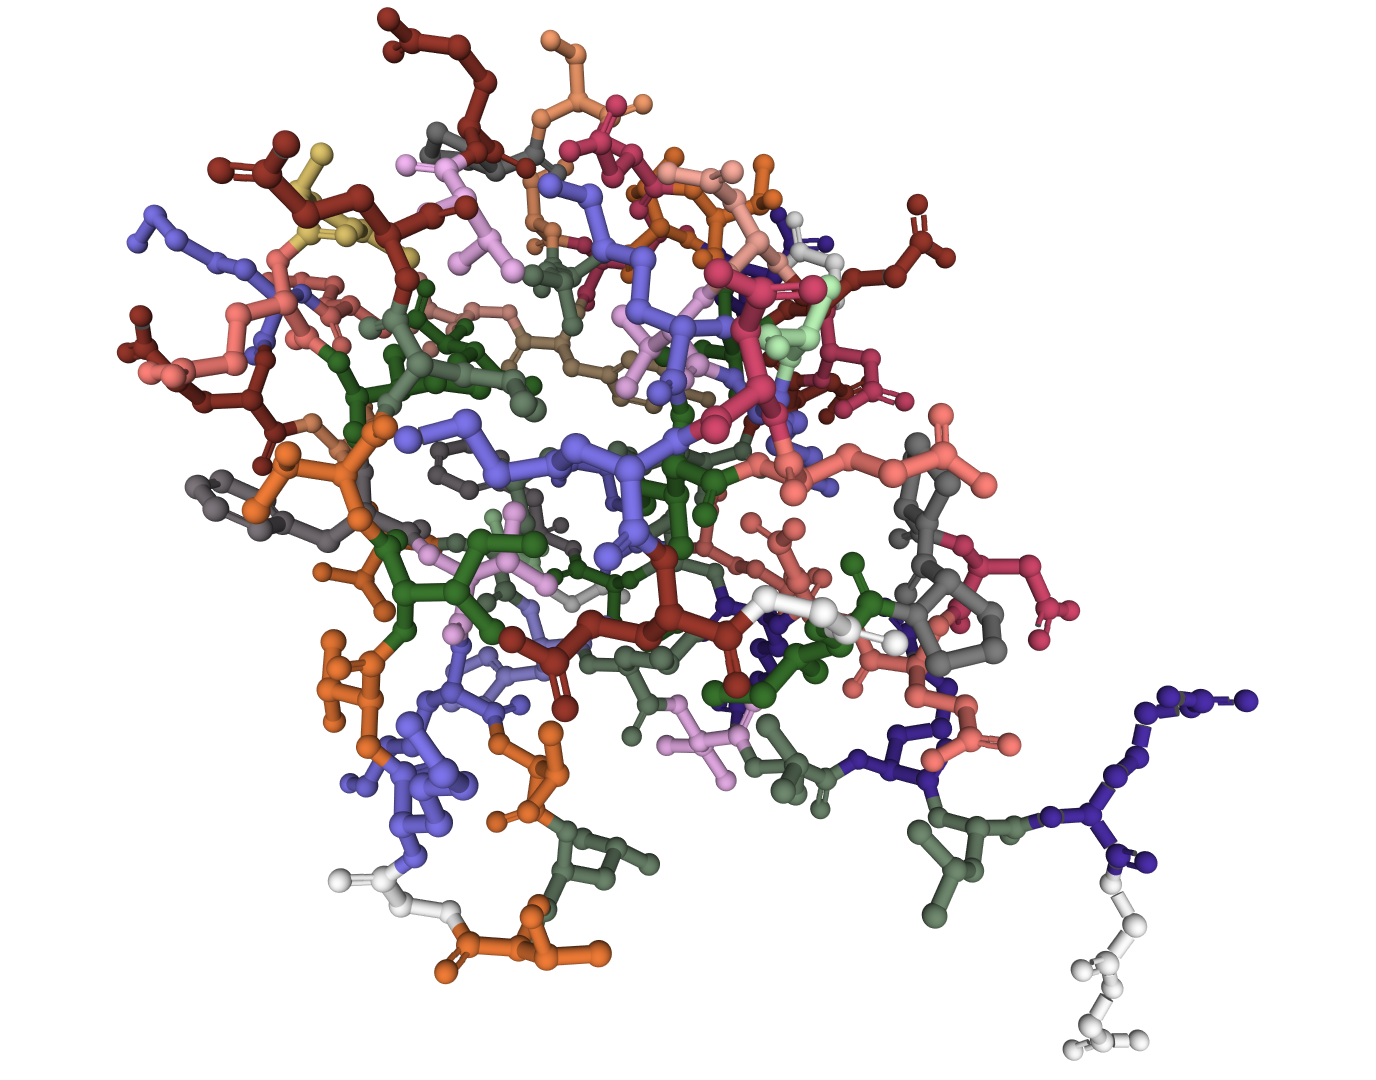
\includegraphics[width = 0.49 \textwidth]{graphics/ubq_balls.png}
  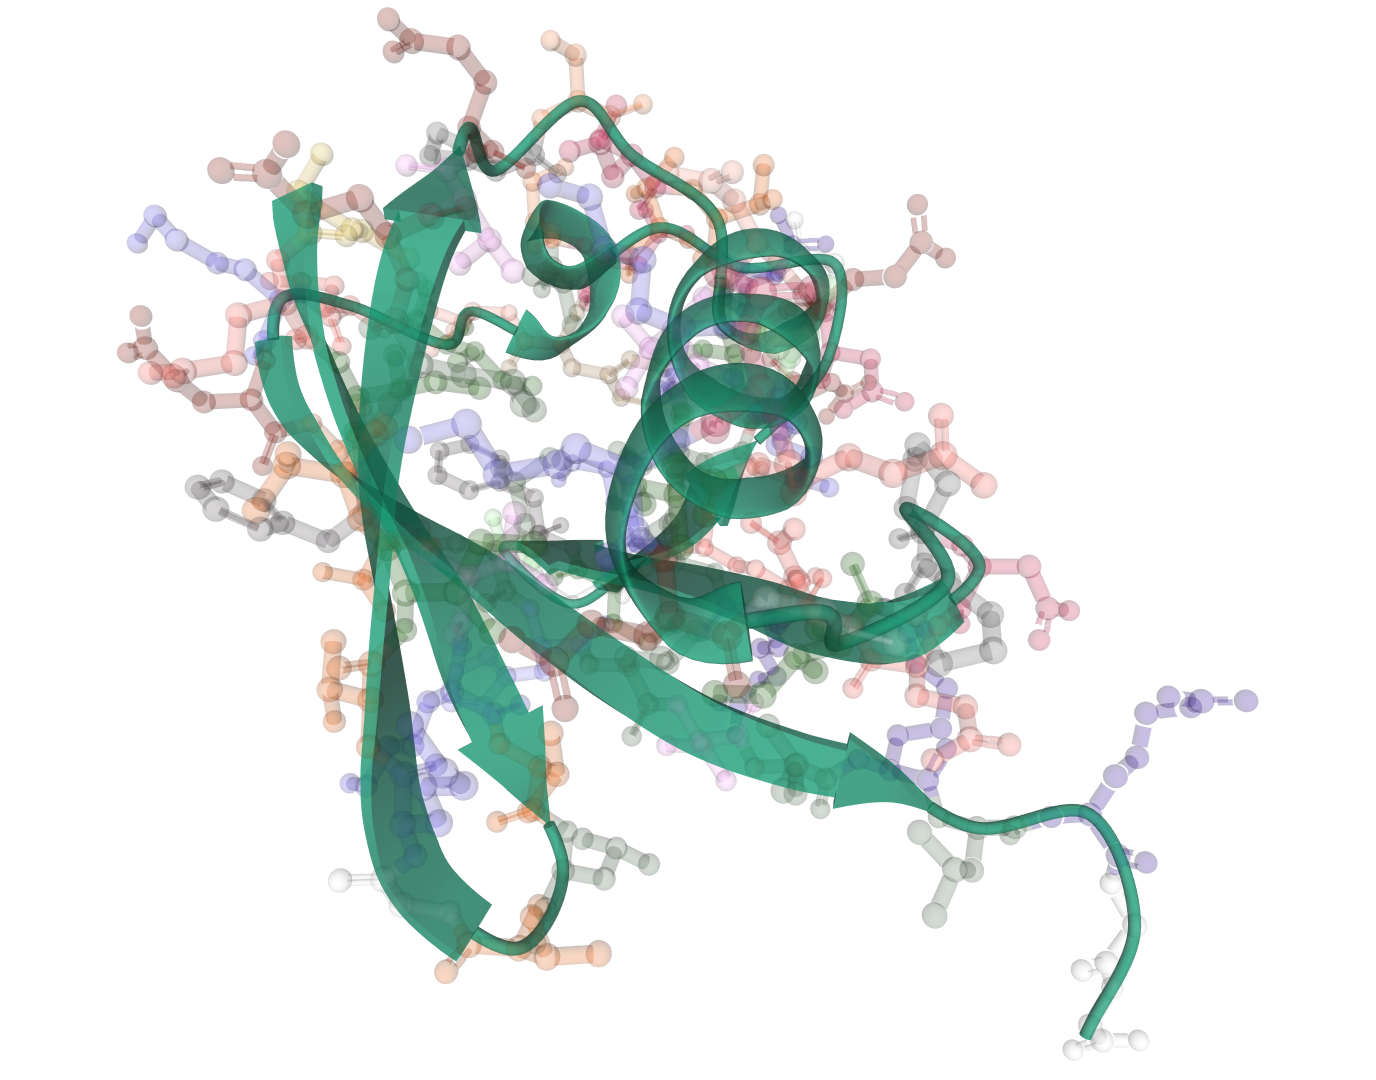
\includegraphics[width = 0.49 \textwidth]{graphics/ubq_ribbon.png}
  \caption{Conformation of ubiquitin. Each ball and stick respectively represent an atom and a covalent bond, colors correspond to residues (left). 
  Additional ribbon diagram highlighting the linear arrangement of residues is superimposed on the atoms (right). 
  Both images were created with Mol*~\cite{mol}.}
  \label{f:ubq}
\end{figure}


Molecular dynamics (MD) simulations offer a promising approach to deriving dynamics of a protein
from easily obtainable information, such as its amino acid sequence. 
In a traditional MD algorithm, which dates back to the 70s~\cite{md_nature}, positions and velocities
of all atoms forming the protein are maintained explicitly. In subsequent steps they are updated 
by numerically integrating equations of motion. Those equations often boil down to calculating the net
force acting on each atom and simply applying Newton's second law of motion~\cite{md_aa}. 
The core of any MD model is defining force fields that govern how the atoms interact with each other
and fine-tuning them so that the results match experimental data.

The most limiting factor of MD simulations is reaching time scales relevant to biological processes.
During each step we can advance time by only so much before introducing artifacts and instability.
This usually limits the time step to the order of $10^{-15}$ seconds, which is $10^9$ times smaller than 
even the shortest relevant simulation lengths~\cite{md_aa}. 
Because of this limitation a single MD experiment can take many days or even weeks to finish 
and any significant speed-up of the algorithm's implementation would increase its range of applications. 

An example method of increasing available simulation time scales is to use coarse-grained representation of a protein. 
This requires dividing atoms into groups, e.g. by amino acid residue they come from, and then treating each group as one object. 
This can decrease the amount of computation required to process one step, but the biggest profit is that  
because of losing some details about the movement of individual atoms, we can greatly increase the time step 
before running into issues with stability~\cite{md_aa}. However, this comes at a cost of reduced accuracy
and increased complexity of the model and its implementation.


As part of this thesis we have reimplemented a coarse-grained MD model developed in the Institute of Physics of the Polish Academy of Sciences. The model and its implementation have been developed for over 20 years, starting in 2000 with a first version created to simulate ordered proteins~\cite{cg_1}, i.e. proteins that have a known, stable conformation. Then, in 2008, it was used to study stretching of proteins~\cite{cg_2} and lately, in 2018, extended to also simulate disordered proteins~\cite{QA_model}, which may have no stable conformation. In 2020, a more accurate method for disordered proteins was developed~\cite{PID}. The program in its current state has many flaws, the most important being that it's overcomplicated, which makes it hard to understand and even harder to extend with new functionalities. Some of this complexity comes from the model itself, but arguably most of it comes from poor programming practices and an obsolete programming language (FORTRAN 77), which doesn't provide enough high-level abstractions needed for such complex application. The authors of the program realized that it would be beneficial to reimplement this model in a modern, high-level language and this thesis is a summary of our efforts to produce readable, efficient and functionally equivalent code.


The rest of this thesis is organized as follows: In chapter 2, we provide basic information about the model itself. In chapter 3, we discuss the original implementation, list some of its features and comment on its issues, this way we provide justification for the project and make it possible to later argue why the new implementation is qualitatively better. Chapter 4 is the focal point of this thesis, it presents the new design as well as comparison of how the features are implemented in both programs. It also describes how we achieve better parallelism and discusses some new interesting optimizations. Chapter 5 contains some benchmarks' results and their analysis --- these provide the most objective advantages of the new program over the old one. In chapter 6 we give an overview of individual contributions among the team and in chapter 7 we describe additional files attached to this thesis. 